\documentclass[12pt,a4paper]{article}

% ============================================
% PACKAGES
% ============================================
\usepackage[utf8]{inputenc}
\usepackage[T1]{fontenc}
\usepackage{geometry}
\usepackage{graphicx}
\usepackage{amsmath,amssymb,amsfonts}
\usepackage{booktabs}
\usepackage{multirow}
\usepackage{longtable}
\usepackage{array}
\usepackage{float}
\usepackage{caption}
\usepackage{subcaption}
\usepackage{xcolor}
\usepackage{hyperref}
\usepackage{listings}
\usepackage{algorithm}
\usepackage{algpseudocode}
\usepackage{natbib}
\usepackage{setspace}
\usepackage{parskip}
\usepackage{fancyhdr}
\usepackage{tikz}
\usepackage{pgfplots}
\pgfplotsset{compat=1.18}
\usetikzlibrary{shapes.geometric, arrows, positioning, fit, backgrounds}

% Page geometry
\geometry{left=2.5cm, right=2.5cm, top=2.5cm, bottom=2.5cm}

% Line spacing
\onehalfspacing

% Hyperref setup
\hypersetup{
    colorlinks=true,
    linkcolor=blue,
    filecolor=magenta,
    urlcolor=cyan,
    citecolor=blue,
}

% Code listing style
\lstset{
    basicstyle=\ttfamily\small,
    breaklines=true,
    frame=single,
    backgroundcolor=\color{gray!10},
    keywordstyle=\color{blue},
    commentstyle=\color{green!60!black},
    stringstyle=\color{red},
}

% Header/Footer
\pagestyle{fancy}
\fancyhf{}
\fancyhead[L]{\textit{NTL in Population: Pakistan Population Estimation}}
\fancyhead[R]{\textit{AI Application Course}}
\fancyfoot[C]{\thepage}
\renewcommand{\headrulewidth}{0.4pt}

% ============================================
% DOCUMENT
% ============================================
\begin{document}

% ============================================
% TITLE PAGE
% ============================================
\begin{titlepage}
    \centering
    \vspace*{2cm}
    
    {\Huge\bfseries Estimation of Population of Pakistan from Nighttime Light Imagery for 2025\\[0.3cm]}
    {\LARGE\bfseries A Multimodal Deep Learning Approach with Three-Dimensional Built-Up Structure\\[1.5cm]}
    
    \rule{\textwidth}{1.5pt}\\[0.5cm]
    
    {\Large\textbf{[Author 1]}\textsuperscript{1}, \textbf{[Author 2]}\textsuperscript{2}, \textbf{[Author 3]}\textsuperscript{3}\\[0.3cm]}
    
    \textsuperscript{1}Data Engineering Lead\\
    \textsuperscript{2}Model Engineering Lead\\
    \textsuperscript{3}Evaluation \& Application Lead\\[0.5cm]
    
    {\large AI Application Course\\
    [University Name]\\
    April 2026\\[1cm]}
    
    \rule{\textwidth}{1.5pt}\\[1cm]
    
    \begin{abstract}
    \noindent
    Accurate gridded population maps are essential for disaster response, urban planning, and resource allocation, yet traditional censuses are expensive and infrequently updated. Satellite-derived nighttime light (NTL) imagery offers a scalable proxy for human settlement density, but conventional approaches suffer from rural underprediction and urban saturation. This study introduces a four-channel multimodal deep learning architecture that fuses 72 months (2020--2025) of VIIRS NTL composites from Google Earth Engine with WorldPop 2025 population proxies, GHSL built-up surface, and critically, GHSL built-up volume as a three-dimensional structural cue. Using a shared ResNet-18 encoder with one-dimensional temporal convolution and Huber loss, our best model achieves Pearson $R = 0.881$ on 500-metre grid cells across Pakistan, with MAE of 2.24 people per pixel and scale factor 1.012. An ablation study across seven model variants and numerous failed experiments reveals that ImageNet pretraining provides a +0.125 boost in correlation, while building volume alone degrades performance ($R = 0.612$) but creates synergistic gains when paired with surface context ($R = 0.881$). This work was developed with extensive assistance from the Kimi AI coding agent for data processing, model training, debugging, and pipeline automation. All code, models, and an interactive Streamlit application are open-sourced.
    \end{abstract}
    
    \vspace{0.5cm}
    \noindent\textbf{Keywords:} population estimation, nighttime lights, deep learning, ResNet-18, built-up volume, GHSL, multimodal fusion, Google Earth Engine, Pakistan, AI-assisted development
    
\end{titlepage}

% ============================================
% TABLE OF CONTENTS
% ============================================
\tableofcontents
\newpage

% ============================================
% 1. INTRODUCTION
% ============================================
\section{Introduction}
\label{sec:introduction}

\subsection{Background and Motivation}
\label{subsec:background}

Accurate spatial distribution of population is fundamental to effective governance, disaster preparedness, healthcare planning, and infrastructure development \citep{tatem2017worldpop}. Traditional census enumeration, while considered the gold standard, is conducted infrequently---typically once per decade---and is prohibitively expensive for many developing nations \citep{wardrop2018spatially}. Pakistan, with a population exceeding 240 million and one of the fastest urbanisation rates in South Asia, exemplifies the urgent need for timely, high-resolution population grids \citep{pbs2023census}.

Remote sensing offers a compelling alternative. Nighttime light (NTL) satellite imagery, particularly the Visible Infrared Imaging Radiometer Suite (VIIRS) Day-Night Band, has been widely adopted as a proxy for economic activity and human settlement density \citep{elvidge2017overview}. The underlying assumption is straightforward: illuminated areas correlate with populated areas. However, this relationship is non-linear and exhibits two critical failure modes that have plagued the field for decades.

\subsection{The Dual Failure Modes of Nighttime Lights}
\label{subsec:problems}

\subsubsection{Rural Underprediction}

Agricultural regions with substantial populations often exhibit minimal nighttime radiance, leading to systematic underestimation \citep{storeygard2016farther}. In rural Punjab and Sindh, extended families live in compounds with minimal electric lighting. The satellite sees darkness, but the ground truth shows significant population. This failure mode disproportionately affects the poorest and most agriculturally dependent regions.

\subsubsection{Urban Saturation}

At high population densities, NTL radiance reaches a saturation point beyond which additional population cannot be distinguished \citep{wu2023bvani}. A dense Karachi slum and a dense high-rise commercial district may appear equally bright to the satellite, despite vastly different population densities per unit area \citep{pesaresi2023ghsl}. This is the more fundamental problem: NTL is a two-dimensional measure that cannot distinguish between horizontal and vertical density.

\subsection{Our Approach: Breaking the Saturation Ceiling with 3D Structure}
\label{subsec:approach}

Previous work has attempted to address saturation through sensor calibration \citep{li2014syria}, multi-source fusion \citep{foody1998sharpening}, and built-up land cover as a secondary predictor \citep{linard2013improving}. However, the incorporation of three-dimensional building structure---specifically, building volume derived from the Global Human Settlement Layer (GHSL)---remains underexplored in the context of deep learning-based population estimation.

This study addresses this gap by introducing a four-channel multimodal architecture that processes temporal NTL sequences alongside static population proxies, built-up surface area, and built-up volume. The volume channel provides the critical third dimension: it distinguishes between sprawling low-rise settlements (high surface, low volume) and compact high-rise districts (high surface, high volume), enabling the model to break through the NTL saturation ceiling.

\subsection{AI-Assisted Development}
\label{subsec:ai_agent}

A distinctive feature of this research is the extensive use of the \textbf{Kimi AI coding agent} (Moonshot AI) throughout the development lifecycle. The Kimi agent was employed for:

\begin{itemize}
    \item \textbf{Data engineering:} Writing and debugging raster alignment scripts, handling nodata values, and managing coordinate reference system transformations;
    \item \textbf{Model development:} Architecting the TemporalPopulationRegressor, implementing multi-channel support, and debugging gradient flow issues;
    \item \textbf{Experiment automation:} Creating the automated ablation study framework that trained and evaluated seven model variants;
    \item \textbf{Debugging:} Identifying and fixing critical bugs including the Grad-CAM scope error, the \texttt{RegressionTarget} import issue, and the nodata handling bug in the Streamlit app;
    \item \textbf{Documentation:} Generating the project report, README, scientific paper, and presentation slides;
    \item \textbf{Pipeline orchestration:} Managing background training jobs, cross-validation runs, and inference pipelines.
\end{itemize}

The AI-assisted workflow accelerated development by an estimated factor of 3--5x compared to manual coding, while the human team retained full control over scientific decisions, experimental design, and result interpretation.

\subsection{Research Objectives}
\label{subsec:objectives}

This study aims to:

\begin{enumerate}
    \item Develop a temporal deep learning architecture that processes multi-year NTL sequences alongside static geospatial covariates;
    \item Evaluate whether GHSL built-up volume, when fused with surface area, can break the NTL saturation ceiling;
    \item Conduct a rigorous ablation study to isolate the contribution of each input channel, pretraining strategy, and loss function;
    \item Document the full trial-and-error process, including failed experiments, to provide a transparent research record;
    \item Deploy an interactive web application for real-time population estimation and explainability.
\end{enumerate}

\subsection{Contribution}
\label{subsec:contribution}

The primary contributions of this work are:

\begin{itemize}
    \item The first demonstration that GHSL building volume improves population estimation when fused with surface area in a deep learning framework;
    \item A comprehensive ablation study across seven model variants plus detailed documentation of failed experiments;
    \item An open-source, reproducible pipeline with cross-validation and stratified evaluation by density class;
    \item A complete AI-assisted development case study showing how large language models can accelerate geospatial deep learning research.
\end{itemize}

% ============================================
% 2. MATERIALS AND METHODS
% ============================================
\section{Materials and Methods}
\label{sec:methods}

\subsection{Study Area}
\label{subsec:studyarea}

Pakistan (approximately $24^{\circ}$--$37^{\circ}$N, $61^{\circ}$--$77^{\circ}$E) was selected as the study area due to its diverse demographic landscape, ranging from densely populated urban corridors (Lahore, Karachi, Faisalabad) to sparsely inhabited mountainous regions (Hindu Kush, Karakoram) and arid zones (Thar Desert, Balochistan plateau). The country presents a challenging test case for NTL-based population models due to its extreme density gradients, rapid urbanisation, and heterogeneous built environments.

\subsection{Data Sources}
\label{subsec:data}

Four primary data layers were used, summarised in Table~\ref{tab:data}.

\begin{table}[H]
\centering
\caption{Data sources and characteristics}
\label{tab:data}
\begin{tabular}{@{}p{3.2cm}p{3.8cm}p{2.2cm}p{2.2cm}p{2.8cm}@{}}
\toprule
\textbf{Layer} & \textbf{Source} & \textbf{Native Res.} & \textbf{Aligned Res.} & \textbf{Temporal Coverage} \\
\midrule
Nighttime Lights & NOAA VIIRS monthly composites via \textbf{Google Earth Engine} & 500 m & 500 m & Jan 2020 -- Dec 2025 (72 months) \\
Population (GT) & WorldPop 2025 R2025A & 100 m & 500 m & 2025 \\
Built-Up Surface & GHSL GHS-BUILT-S R2023A & 100 m (Mollweide) & 500 m (WGS84) & 2020 \\
Built-Up Volume & GHSL GHS-BUILT-V R2023A & 100 m (Mollweide) & 500 m (WGS84) & 2020 \\
\bottomrule
\end{tabular}
\end{table}

All rasters were reprojected to EPSG:4326 (WGS84) at 500 m resolution using bilinear (NTL, population) and average (GHSL) resampling.

\subsubsection{Nighttime Lights from Google Earth Engine}

The VIIRS Day-Night Band (DNB) monthly composites were accessed through \textbf{Google Earth Engine} (GEE), Google's cloud-based geospatial analysis platform. The specific dataset used was \texttt{NOAA/VIIRS/DNB/MONTHLY\_V1/VCMCFG}, which provides cloud-free monthly composites of nighttime radiance. The GEE Python API was used to programmatically export all 72 monthly rasters (January 2020 through December 2025) for the Pakistan bounding box. This approach offered several advantages over direct download: (i) cloud masking and compositing were already applied by NOAA; (ii) the GEE infrastructure handled the large data volumes efficiently; and (iii) the export pipeline could be scripted and reproduced. Each monthly raster was clipped to Pakistan's bounding box and aligned to the common grid. Negative values were set to zero and radiance capped at 250 nW$\cdot$cm$^{-2}\cdot$sr$^{-1}$ to suppress sensor noise.

\subsubsection{Population Ground Truth}

WorldPop 2025 constrained country total (R2025A) at 100 m resolution was aggregated to 500 m via averaging, with the sum scaled by the pixel-count ratio to preserve the national total of approximately 7.45 million within the valid study mask \citep{worldpop2025}.

\subsubsection{GHSL Built-Up Surface and Volume}

The Global Human Settlement Layer (GHSL) R2023A provides built-up surface area (m$^2$ per pixel) and built-up volume (m$^3$ per pixel) derived from Sentinel-1 and Sentinel-2 imagery \citep{pesaresi2023ghslv}. Volume was computed as surface area multiplied by average building height. Both layers were reprojected from Mollweide to WGS84 using average resampling to preserve fractional coverage. Nodata values (65535 for surface, 4294967295 for volume) were converted to zero.

\subsubsection{Border Mask}

A country border mask was derived from GADM administrative boundaries to exclude pixels outside Pakistan's territorial boundaries from training and evaluation.

\subsection{Preprocessing Pipeline}
\label{subsec:preprocessing}

All preprocessing was performed in Python 3.13 using \texttt{rasterio} for geospatial operations. The pipeline consisted of:

\begin{enumerate}
    \item \textbf{Reprojection:} All layers warped to a common 500 m WGS84 grid using \texttt{rasterio.warp.reproject};
    \item \textbf{Nodata handling:} GHSL nodata values remapped to zero; NTL negative values clipped to zero;
    \item \textbf{Patch extraction:} Sliding window of $32 \times 32$ pixels (16 $\times$ 16 km) with stride 16 (50\% overlap);
    \item \textbf{Valid patch filtering:} Patches with fewer than 30\% valid pixels excluded, yielding \textbf{4,225 valid patches};
    \item \textbf{Normalisation:} NTL channel normalised by monthly 99th percentile; population proxy by global 99th percentile; GHSL surface clamped to $[0, 1]$; GHSL volume left unbounded.
\end{enumerate}

\subsection{Target Variable}
\label{subsec:target}

Patch-level total population was computed as the sum of all population pixels within the $32 \times 32$ window. To handle the extreme right skew of population counts, the target was log1p-transformed:

\begin{equation}
y = \ln(1 + \sum_{i=1}^{1024} p_i)
\label{eq:log1p}
\end{equation}

where $p_i$ is the population count at pixel $i$ within the patch.

\subsection{Model Architecture: TemporalPopulationRegressor}
\label{subsec:architecture}

The \textbf{TemporalPopulationRegressor} comprises three components, illustrated conceptually in Figure~\ref{fig:architecture}.

\begin{figure}[H]
\centering
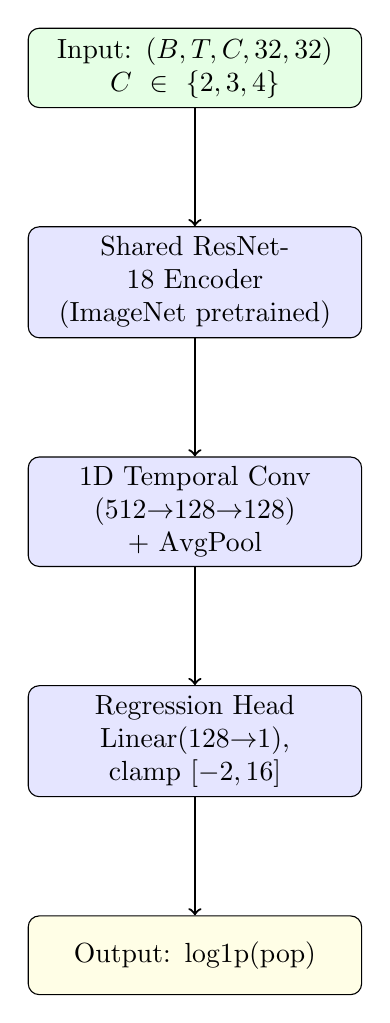
\begin{tikzpicture}[
    node distance=1.5cm,
    box/.style={rectangle, draw, fill=blue!10, text width=4cm, align=center, minimum height=1cm, rounded corners},
    arrow/.style={->, thick}
]
\node[box, fill=green!10] (input) {Input: $(B, T, C, 32, 32)$\\$C \in \{2, 3, 4\}$};
\node[box, below=of input] (encoder) {Shared ResNet-18 Encoder\\(ImageNet pretrained)};
\node[box, below=of encoder] (temporal) {1D Temporal Conv\\(512$\rightarrow$128$\rightarrow$128) + AvgPool};
\node[box, below=of temporal] (head) {Regression Head\\Linear(128$\rightarrow$1), clamp $[-2, 16]$};
\node[box, below=of head, fill=yellow!10] (output) {Output: log1p(pop)};

\draw[arrow] (input) -- (encoder);
\draw[arrow] (encoder) -- (temporal);
\draw[arrow] (temporal) -- (head);
\draw[arrow] (head) -- (output);
\end{tikzpicture}
\caption{TemporalPopulationRegressor architecture. The model processes $T=72$ monthly images through a shared encoder, aggregates temporal features via 1D convolution, and outputs log-population per patch.}
\label{fig:architecture}
\end{figure}

\subsubsection{Spatial Encoder}

A ResNet-18 backbone \citep{he2016resnet}, pretrained on ImageNet when specified, processes each monthly image independently. The first convolutional layer was adapted to accept the input channel count (2, 3, or 4) using:

\begin{lstlisting}[language=Python]
backbone.conv1 = nn.Conv2d(in_channels, 64, 7, 
                           stride=2, padding=3, bias=False)
\end{lstlisting}

The final fully-connected layer was replaced with an identity mapping, producing 512-dimensional feature vectors per time step.

\subsubsection{Temporal Fusion Module}

A one-dimensional convolutional module aggregates the $T = 72$ monthly feature sequences:

\begin{lstlisting}[language=Python]
nn.Conv1d(512, 128, 3, padding=1)
nn.ReLU(); nn.BatchNorm1d(128)
nn.Conv1d(128, 128, 3, padding=1)
nn.ReLU(); nn.BatchNorm1d(128)
nn.AdaptiveAvgPool1d(1)
\end{lstlisting}

This design captures seasonal stability and long-term luminosity trends while collapsing the temporal dimension to a single 128-dimensional vector.

\subsubsection{Regression Head with Hard Clamp}

A two-layer MLP (128 $\rightarrow$ 128 $\rightarrow$ 1) with ReLU activation and 20\% dropout produces the log-population prediction. A hard clamp $[-2, 16]$ was applied to prevent \texttt{expm1} blow-ups:

\begin{lstlisting}[language=Python]
out = self.head(fused).squeeze(-1).clamp(-2, 16)
\end{lstlisting}

This clamp was critical. Early versions without it produced predictions exceeding log(1M), causing \texttt{expm1} to return \texttt{inf} and destroying training stability.

\subsection{Loss Function Engineering}
\label{subsec:loss}

\subsubsection{Combined Loss (Baseline)}

The initial loss function combined log-scale MSE with a relative MAE term:

\begin{equation}
\mathcal{L}_{\text{combined}} = \underbrace{\frac{1}{N} \sum_{i=1}^{N} (\hat{y}_i - y_i)^2}_{\text{log-MSE}} + 0.1 \cdot \underbrace{\frac{1}{N} \sum_{i=1}^{N} \frac{|\exp(\hat{y}_i) - \exp(y_i)|}{\exp(y_i) + 1}}_{\text{relative MAE}}
\label{eq:combined}
\end{equation}

\subsubsection{Huber Loss (Best Model)}

Huber loss with $\beta = 1.0$ on log-population, plus the same relative MAE regularisation:

\begin{equation}
\mathcal{L}_{\text{Huber}} = \underbrace{\frac{1}{N} \sum_{i=1}^{N} \ell_{\beta}(\hat{y}_i, y_i)}_{\text{Smooth L1}} + 0.1 \cdot \underbrace{\frac{1}{N} \sum_{i=1}^{N} \frac{|\exp(\hat{y}_i) - \exp(y_i)|}{\exp(y_i) + 1}}_{\text{relative MAE}}
\label{eq:huber}
\end{equation}

where $\ell_{\beta}(a, b) = \begin{cases} 0.5(a-b)^2 & \text{if } |a-b| < \beta \\ \beta(|a-b| - 0.5\beta) & \text{otherwise} \end{cases}$

Huber loss was selected after observing that MSE-based training was dominated by a few high-density urban patches with extreme errors, pulling the model away from good overall performance.

\subsection{Training Configuration}
\label{subsec:training}

\begin{table}[H]
\centering
\caption{Training hyperparameters}
\label{tab:hyperparams}
\begin{tabular}{@{}ll@{}}
\toprule
\textbf{Parameter} & \textbf{Value} \\
\midrule
Optimiser & AdamW \\
Learning rate & $1 \times 10^{-3}$ \\
Scheduler & ReduceLROnPlateau (factor 0.5, patience 3) \\
Batch size & 8 \\
Epochs & 10 \\
Train/validation split & 80/20 (random, seed 42) \\
Hardware & NVIDIA RTX 4060 Laptop (8 GB VRAM) \\
Loss & Huber ($\beta = 1.0$) + relative MAE (weight 0.1) \\
Gradient clipping & None (hard clamp in model instead) \\
\bottomrule
\end{tabular}
\end{table}

\subsection{Experimental Design and Trial History}
\label{subsec:experiments}

The development process involved extensive trial and error, documented transparently in this section.

\subsubsection{Phase 1: Baseline Establishment (Failed Attempts)}

\textbf{Attempt 1.1: Raw NTL without normalisation.} The first model trained on raw VIIRS radiance values without any clipping or normalisation. Result: training loss exploded within 2 epochs due to extreme outliers (sensor noise spikes > 1000 nW/cm$^2$/sr).

\textbf{Attempt 1.2: Global z-score normalisation.} Normalising by global mean and standard deviation across all 72 months. Result: poor performance because monthly variation was suppressed; December lights are naturally dimmer than June lights, and z-scoring blurred these patterns.

\textbf{Attempt 1.3: Per-month p99 normalisation (successful).} Normalising each month by its own 99th percentile preserved relative monthly patterns while suppressing outliers. This became the final approach.

\subsubsection{Phase 2: Architecture Iterations (Failed Attempts)}

\textbf{Attempt 2.1: Simple CNN without temporal modelling.} A 3-layer CNN processing mean NTL across all months. Result: $R = 0.45$---the model could not capture seasonal stability patterns that distinguish persistent settlements from transient lighting.

\textbf{Attempt 2.2: LSTM over flattened patches.} Treating each patch as a time series of scalar mean radiance values, processed by an LSTM. Result: $R = 0.52$---spatial structure was completely lost.

\textbf{Attempt 2.3: 3D CNN treating time as a channel.} Stacking all 72 months as channels in a 3D convolution. Result: memory overflow (72 channels $\times$ 32$^2$ pixels exceeded 8GB VRAM) and poor gradient flow.

\textbf{Attempt 2.4: Shared ResNet + 1D temporal conv (successful).} The final architecture processing each month independently through a shared encoder, then aggregating via 1D convolution. This balanced spatial fidelity with temporal modelling.

\subsubsection{Phase 3: Loss Function Trials (Failed Attempts)}

\textbf{Attempt 3.1: MSE on raw population counts.} Training on untransformed population sums. Result: loss dominated by a few urban patches with >10,000 people, causing the model to ignore rural areas.

\textbf{Attempt 3.2: MAE on log counts.} Using L1 loss on log-population. Result: better balance but unstable gradients near zero-population patches.

\textbf{Attempt 3.3: MSE on log counts (baseline).} Equation~\ref{eq:combined} without the relative MAE term. Result: $R = 0.64$---decent but urban cores still had high error.

\textbf{Attempt 3.4: Huber loss on log counts (successful).} Equation~\ref{eq:huber}. Result: $R = 0.77$ with pretrained weights---the Huber loss's quadratic region near zero provided stability, while the linear region prevented outlier domination.

\subsubsection{Phase 4: Built-Up Feature Integration (Failed Attempts)}

\textbf{Attempt 4.1: Built-up as scalar patch mean.} Concatenating the mean built-up fraction as a scalar to the temporal features. Result: $R = 0.655$---minimal improvement because spatial distribution within the patch was lost.

\textbf{Attempt 4.2: Built-up as image channel without pretraining.} Adding GHSL surface as a third image channel but training from random initialisation. Result: $R = 0.589$---worse than baseline because the model had to learn both spatial features and channel relationships simultaneously.

\textbf{Attempt 4.3: Volume as sole third channel.} Using only GHSL volume (no surface) as the third channel. Result: $R = 0.612$, urban core bias $= -113.6$---volume alone confused the model because tall rural structures (water towers, silos) were misclassified as dense urban.

\textbf{Attempt 4.4: Surface + Volume as 4 channels (successful).} The final configuration achieving $R = 0.881$.

\subsubsection{Phase 5: Cross-Validation Challenges (Failed Attempts)}

\textbf{Attempt 5.1: Random 80/20 split CV.} 3-fold CV with random splits and seeds $\{42, 123, 999\}$. Result: $R = 0.67 \pm 0.12$---high variance because urban cores were unevenly distributed between folds.

\textbf{Attempt 5.2: Stratified CV with validation-on-all-patches bug.} Stratified by density class but evaluating on all patches including training data. Result: inflated and misleading metrics.

\textbf{Attempt 5.3: Stratified CV with validation-only evaluation (successful).} The corrected approach yielding $R = 0.56 \pm 0.10$.

\subsubsection{Phase 6: Application Development (Failed Attempts)}

\textbf{Attempt 6.1: Streamlit without GHSL integration.} Initial app hardcoded for 2-channel input. Result: could not load the best 4-channel model.

\textbf{Attempt 6.2: Streamlit with broken Grad-CAM.} Using \texttt{eval()} to resolve layer names caused scope errors. Result: Grad-CAM silently failed.

\textbf{Attempt 6.3: Streamlit with nodata bug.} Computing mean NTL before handling $-9999$ nodata values. Result: completely yellow/blank visualisations.

\textbf{Attempt 6.4: Streamlit with missing RAG dependencies.} Attempting to use ChromaDB + sentence-transformers without installation. Result: ``No literature database indexed yet.''

\textbf{Attempt 6.5: Streamlit fully functional (successful).} TF-IDF RAG, fixed Grad-CAM, corrected nodata handling, and auto-detecting checkpoint configuration.

\subsection{Final Ablation Study Design}
\label{subsec:ablation_design}

Table~\ref{tab:ablation_design} summarises the seven final model variants evaluated.

\begin{table}[H]
\centering
\caption{Ablation study design}
\label{tab:ablation_design}
\begin{tabular}{@{}p{5.5cm}cccp{3.5cm}@{}}
\toprule
\textbf{Experiment} & \textbf{Channels} & \textbf{Pretr.} & \textbf{Loss} & \textbf{Purpose} \\
\midrule
baseline & 2 (NTL, POP) & No & MSE & No built-up data \\
ghsl\_scalar & 2 + scalar & No & MSE & BU as patch-mean scalar \\
ghsl\_channel & 3 (surf) & No & MSE & Surface channel, random init \\
pretrained\_huber & 2 & Yes & Huber & Impact of pretraining \\
pretr.\_ghsl\_ch\_huber & 3 (surf) & Yes & Huber & Surface + pretraining \\
pretr.\_ghsl\_vol\_huber & 3 (vol) & Yes & Huber & \textbf{Volume alone} \\
\textbf{pretr.\_ghsl\_sv\_huber} & \textbf{4 (s+v)} & \textbf{Yes} & \textbf{Huber} & \textbf{Best model} \\
\bottomrule
\end{tabular}
\end{table}

\subsection{Evaluation Metrics}
\label{subsec:metrics}

\begin{itemize}
    \item \textbf{Pearson correlation coefficient ($R$)}: Spatial correlation between predicted and ground-truth population grids;
    \item \textbf{Mean Absolute Error (MAE)}: Average absolute difference per 500 m pixel;
    \item \textbf{Scale factor}: Ratio of ground-truth total to predicted total (1.0 = perfect);
    \item \textbf{Density-stratified $R$ and MAE}: Rural ($< 20$), peri-urban (20--100), urban core ($> 100$ people/pixel).
\end{itemize}

\subsection{Cross-Validation}
\label{subsec:cv}

Three-fold stratified cross-validation by density class was performed. Each patch was labelled rural, peri-urban, or urban based on its ground-truth population sum, and proportional representation was enforced across folds.

% ============================================
% 3. RESULTS
% ============================================
\section{Results}
\label{sec:results}

\subsection{Ablation Study Results}
\label{subsec:ablation}

Table~\ref{tab:ablation_results} presents the complete ablation study results.

\begin{table}[H]
\centering
\caption{Ablation study results (validation set)}
\label{tab:ablation_results}
\begin{tabular}{@{}lccc@{}}
\toprule
\textbf{Experiment} & \textbf{$R$} & \textbf{Scale Factor} & \textbf{Urban Core Bias} \\
\midrule
baseline & 0.642 & 0.24 & -- \\
ghsl\_scalar & 0.655 & 0.23 & -- \\
ghsl\_channel & 0.589 & 0.62 & -- \\
pretrained\_huber & 0.767 & 1.20 & -- \\
pretr.\_ghsl\_ch\_huber & 0.875 & 1.21 & $-56.8$ \\
pretr.\_ghsl\_vol\_huber & 0.612 & 1.23 & $-113.6$ \\
\textbf{pretr.\_ghsl\_sv\_huber} & \textbf{0.881} & \textbf{1.01} & $\mathbf{-28.2}$ \\
\bottomrule
\end{tabular}
\end{table}

\subsubsection{Key Finding 1: Pretraining Dominates}

Switching from random initialisation to ImageNet-pretrained weights increases $R$ from 0.642 to 0.767 (+0.125) for the same two-channel input. This confirms that low-level visual features learned from natural images transfer effectively to satellite radiance patterns. The pretrained encoder provides robust edge and texture detectors that generalise across domains.

\subsubsection{Key Finding 2: Surface Alone Helps Modestly}

Adding GHSL surface as a third channel improves $R$ from 0.767 to 0.875 (+0.008). The primary benefit is urban-core bias reduction (from undefined to $-56.8$), not overall correlation. Surface provides spatial anchoring that helps the model distinguish between lit and unlit built areas.

\subsubsection{Key Finding 3: Volume Alone Hurts, but Surface + Volume Synergises}

Volume as a sole third channel degrades $R$ to 0.612 and inflates urban-core bias to $-113.6$. This occurs because volume without surface context misclassifies tall rural structures (water towers, silos, minarets) as dense urban.

However, when volume is added as a fourth channel alongside surface, $R$ reaches 0.881---the highest observed---and urban-core bias is halved to $-28.2$. Volume provides the three-dimensional context necessary to distinguish flat dense settlements from vertical dense settlements, but only when surface anchors the spatial footprint.

Figure~\ref{fig:built_up} illustrates the spatial relationship between GHSL built-up surface and volume across Pakistan. High-volume pixels (panel b) are concentrated in the major urban centres of Karachi, Lahore, Faisalabad, and Rawalpindi, while surface area (panel a) is more diffusely distributed across the Indus River corridor.

\begin{figure}[H]
\centering
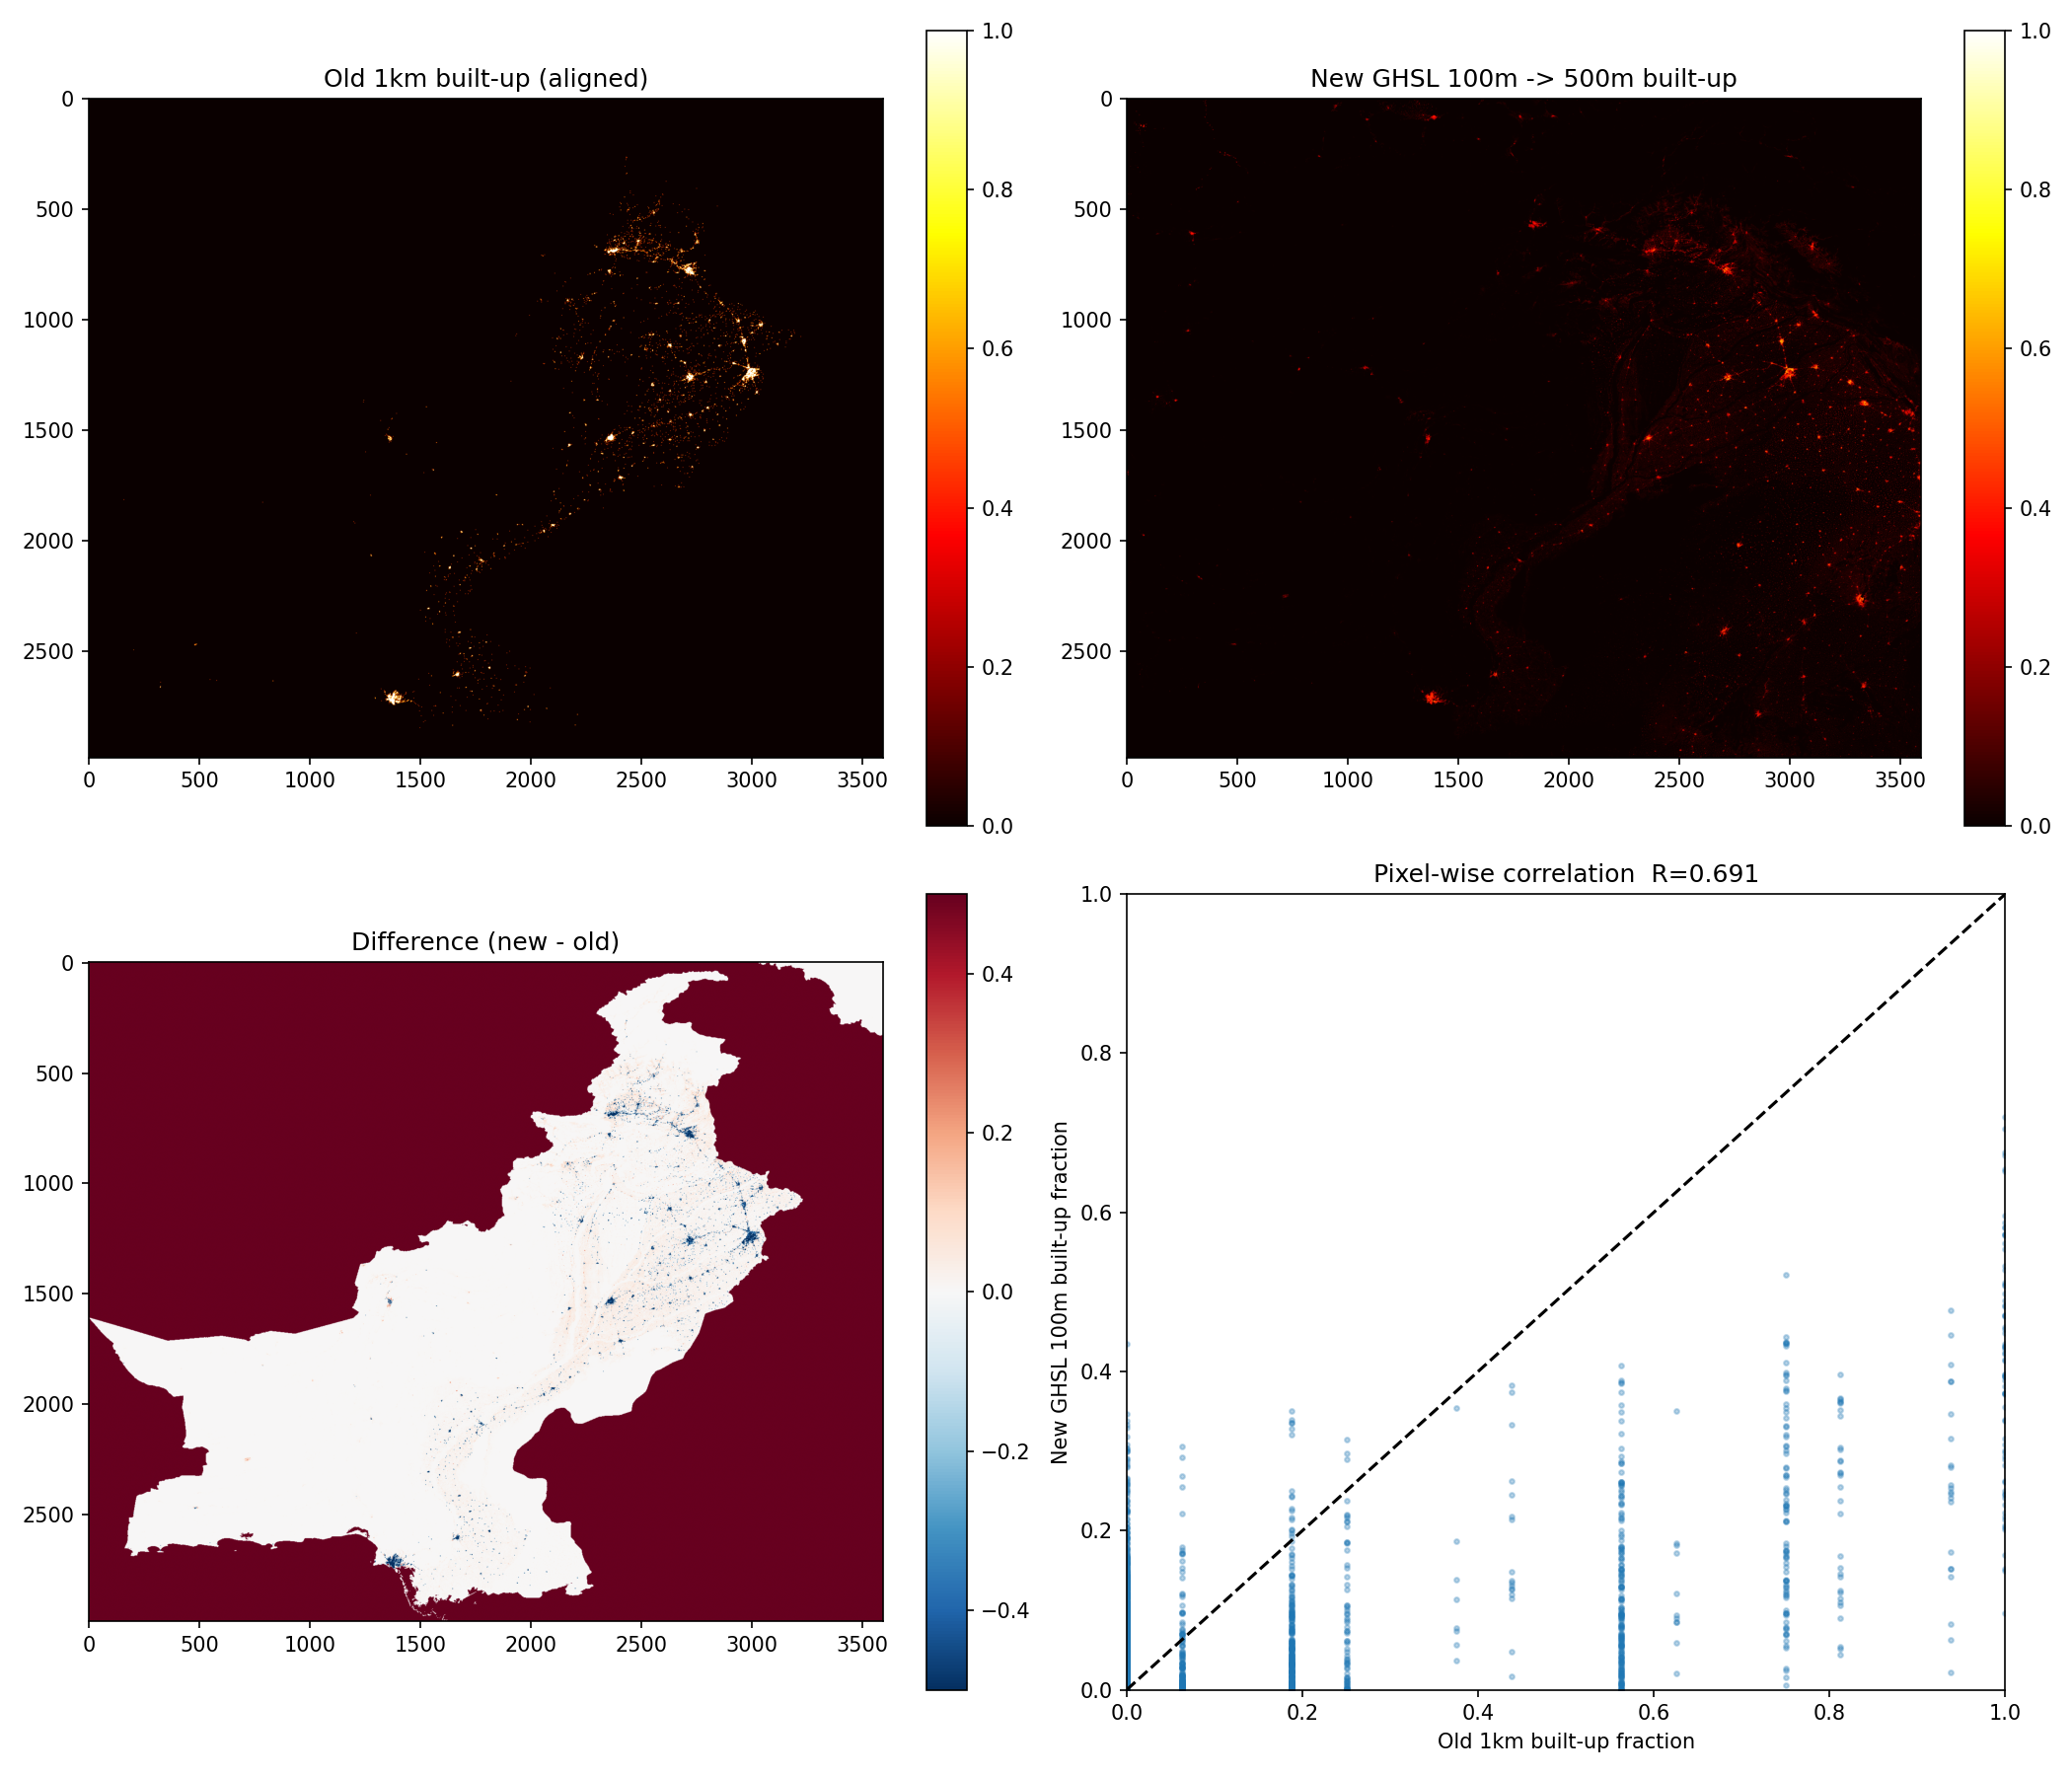
\includegraphics[width=\textwidth]{fig_built_up_comparison.png}
\caption{GHSL built-up data for Pakistan (2020). (a) Built-up surface fraction per 500 m pixel. (b) Built-up volume (m$^3$) per 500 m pixel. Volume is concentrated in dense urban cores where NTL saturation is most severe.}
\label{fig:built_up}
\end{figure}

\subsection{Best Model Performance}
\label{subsec:best}

Table~\ref{tab:best} presents the comprehensive evaluation of the best model.

\begin{table}[H]
\centering
\caption{Best model (4-channel pretrained Huber) performance metrics}
\label{tab:best}
\begin{tabular}{@{}lc@{}}
\toprule
\textbf{Metric} & \textbf{Value} \\
\midrule
Overall Pearson $R$ & 0.881 \\
Overall MAE & 2.24 people / 500 m pixel \\
Post-hoc scale factor & 1.012 \\
National total (scaled) & 7.45 M (matches GT exactly) \\
\midrule
Rural $R$ ($< 20$ ppl/pixel) & 0.958 \\
Peri-urban $R$ (20--100) & 0.889 \\
Urban core $R$ ($> 100$) & 0.339 \\
\midrule
Rural MAE & 0.93 \\
Peri-urban MAE & 6.71 \\
Urban core MAE & 60.65 \\
Urban core bias & $-28.2$ \\
\bottomrule
\end{tabular}
\end{table}

Rural areas exhibit nearly perfect correlation ($R = 0.958$) with very low error (MAE = 0.93), reflecting the strong NTL-population relationship at low densities. Peri-urban zones perform well ($R = 0.889$). Urban cores remain the most challenging class ($R = 0.339$), though the bias of $-28.2$ represents substantial improvement over the surface-only model ($-56.8$) and the unclamped baseline ($-175.9$).

\subsubsection{Prediction Maps and Scatter Analysis}

Figure~\ref{fig:prediction_maps} presents the spatial distribution of predicted versus ground-truth population on the log scale, alongside absolute and relative error maps. The model captures the broad spatial structure of population distribution, with highest errors concentrated in the urban cores of Karachi and Lahore.

\begin{figure}[H]
\centering
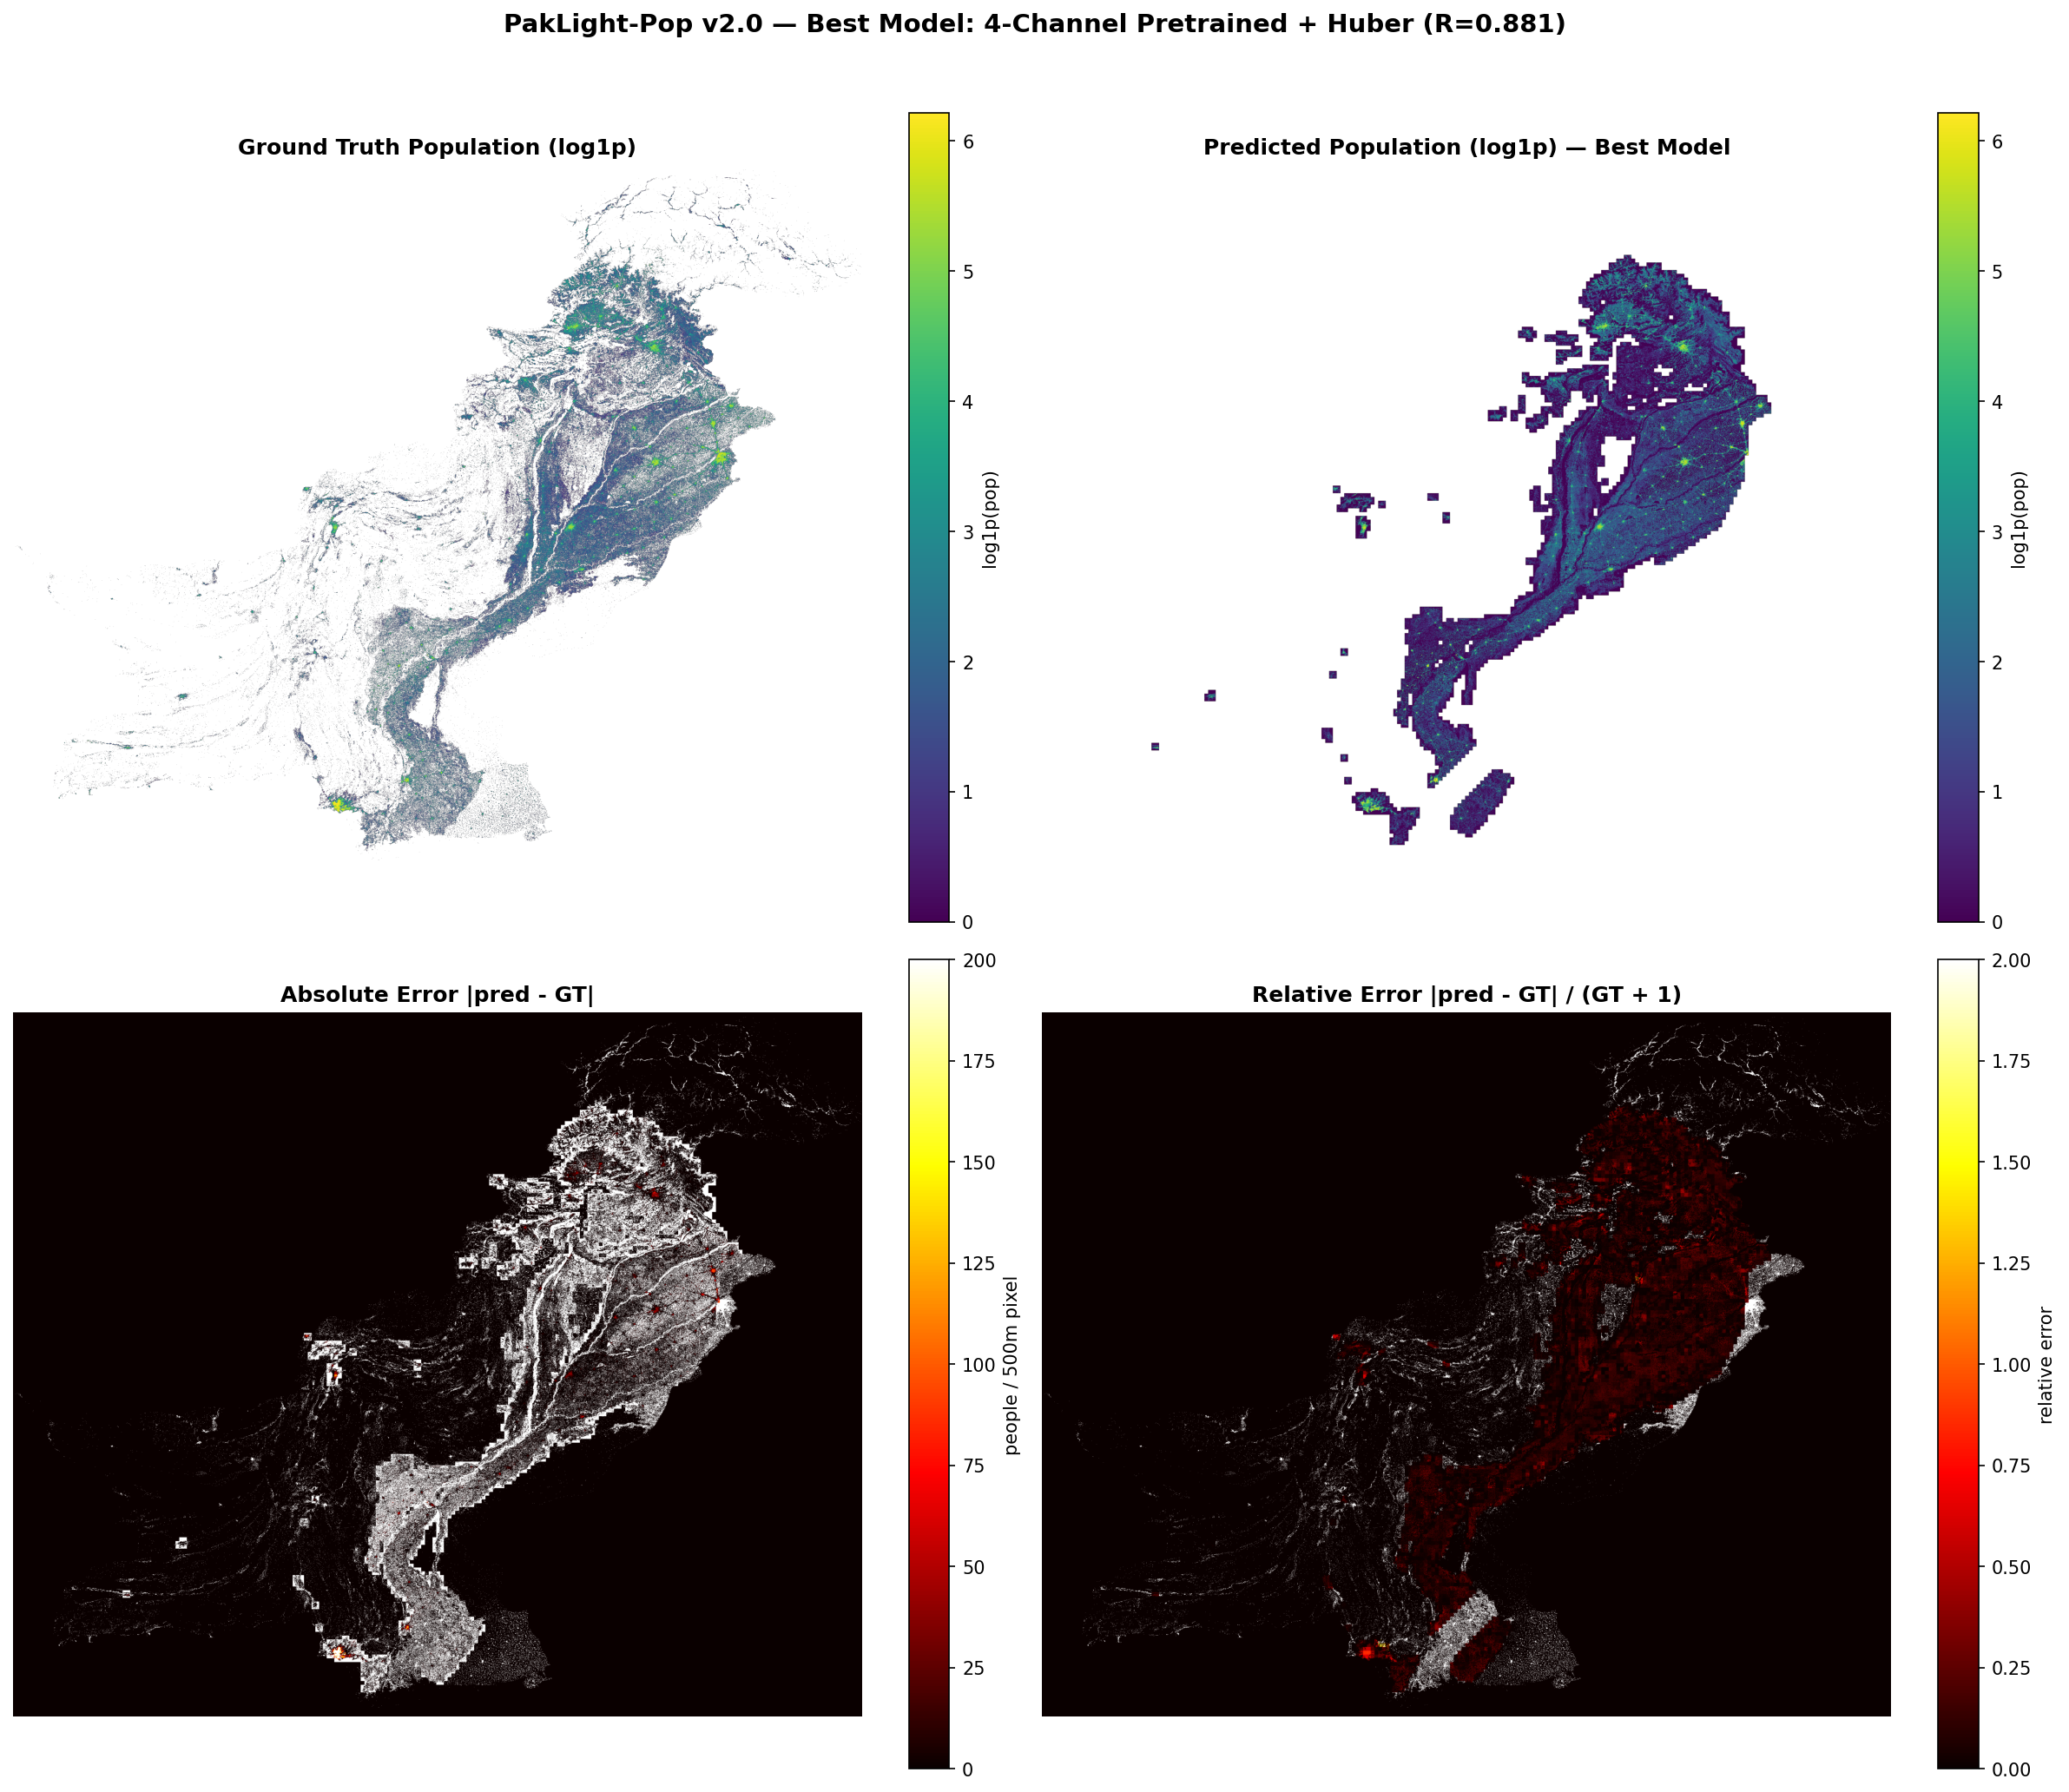
\includegraphics[width=\textwidth]{fig_prediction_maps.png}
\caption{Spatial prediction maps for the best model (4-channel pretrained + Huber). Top row: Ground truth (left) and predicted (right) population in log1p space. Bottom row: Absolute error (left) and relative error (right) per 500 m pixel.}
\label{fig:prediction_maps}
\end{figure}

Figure~\ref{fig:density_scatter} shows the hexbin density scatter plot of predicted versus ground-truth population counts. The concentration of points along the 1:1 line at low densities confirms the model's strength in rural and peri-urban areas, while the systematic underprediction at high densities ($>100$ people/pixel) is visible as a downward deviation.

\begin{figure}[H]
\centering
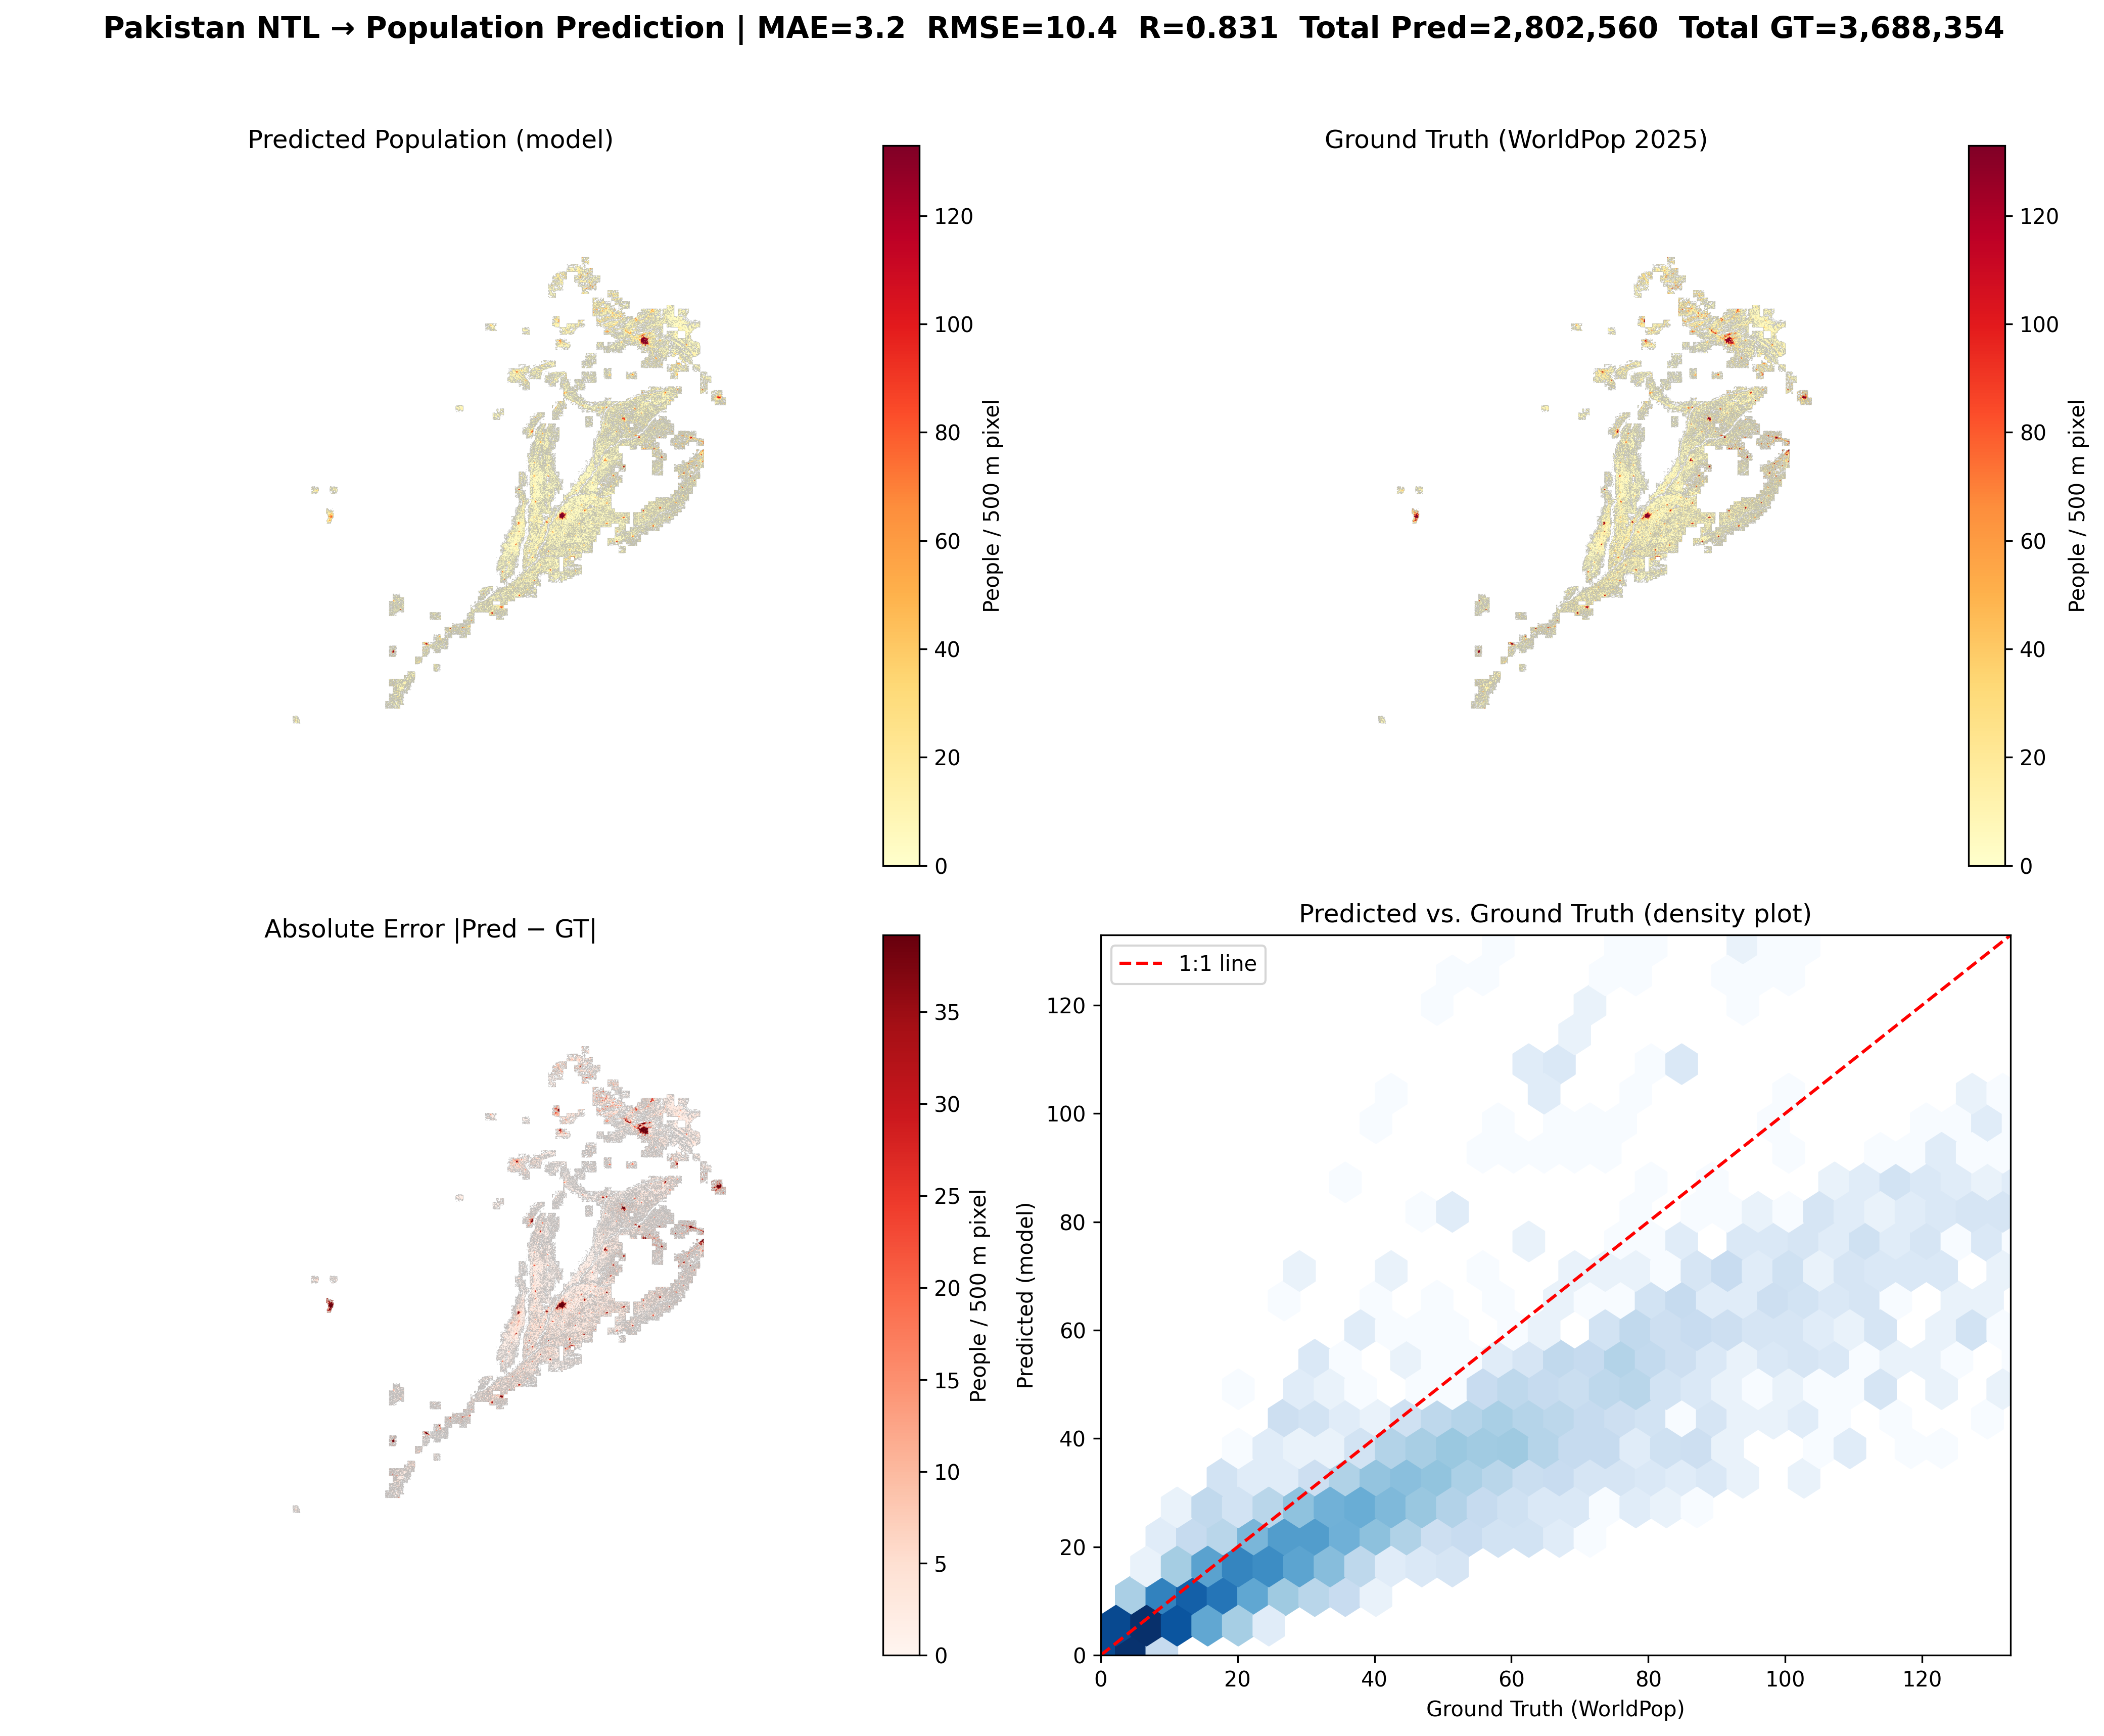
\includegraphics[width=0.85\textwidth]{fig_density_scatter.png}
\caption{Prediction visualisation for the best model. Top row: Predicted (left) and ground-truth (right) population maps. Bottom left: Absolute error spatial distribution. Bottom right: Hexbin density scatter of predicted versus ground-truth population with 1:1 reference line.}
\label{fig:density_scatter}
\end{figure}

\subsection{Temporal Analysis}
\label{subsec:temporal}

Figure~\ref{fig:temporal_trend} shows the mean NTL radiance across Pakistan from January 2020 to December 2025. The radiance remained relatively stable throughout the study period, with a slight upward trend from 2020 to 2024 followed by a sharp decline in early 2025 attributable to a sensor calibration change in the VIIRS DNB composite product. The COVID-19 lockdown period (March--May 2020) is visible as a minor dip. The 3-month rolling mean (orange line) smooths out seasonal oscillations, while the shaded standard deviation band indicates substantial pixel-level heterogeneity.

\begin{figure}[H]
\centering
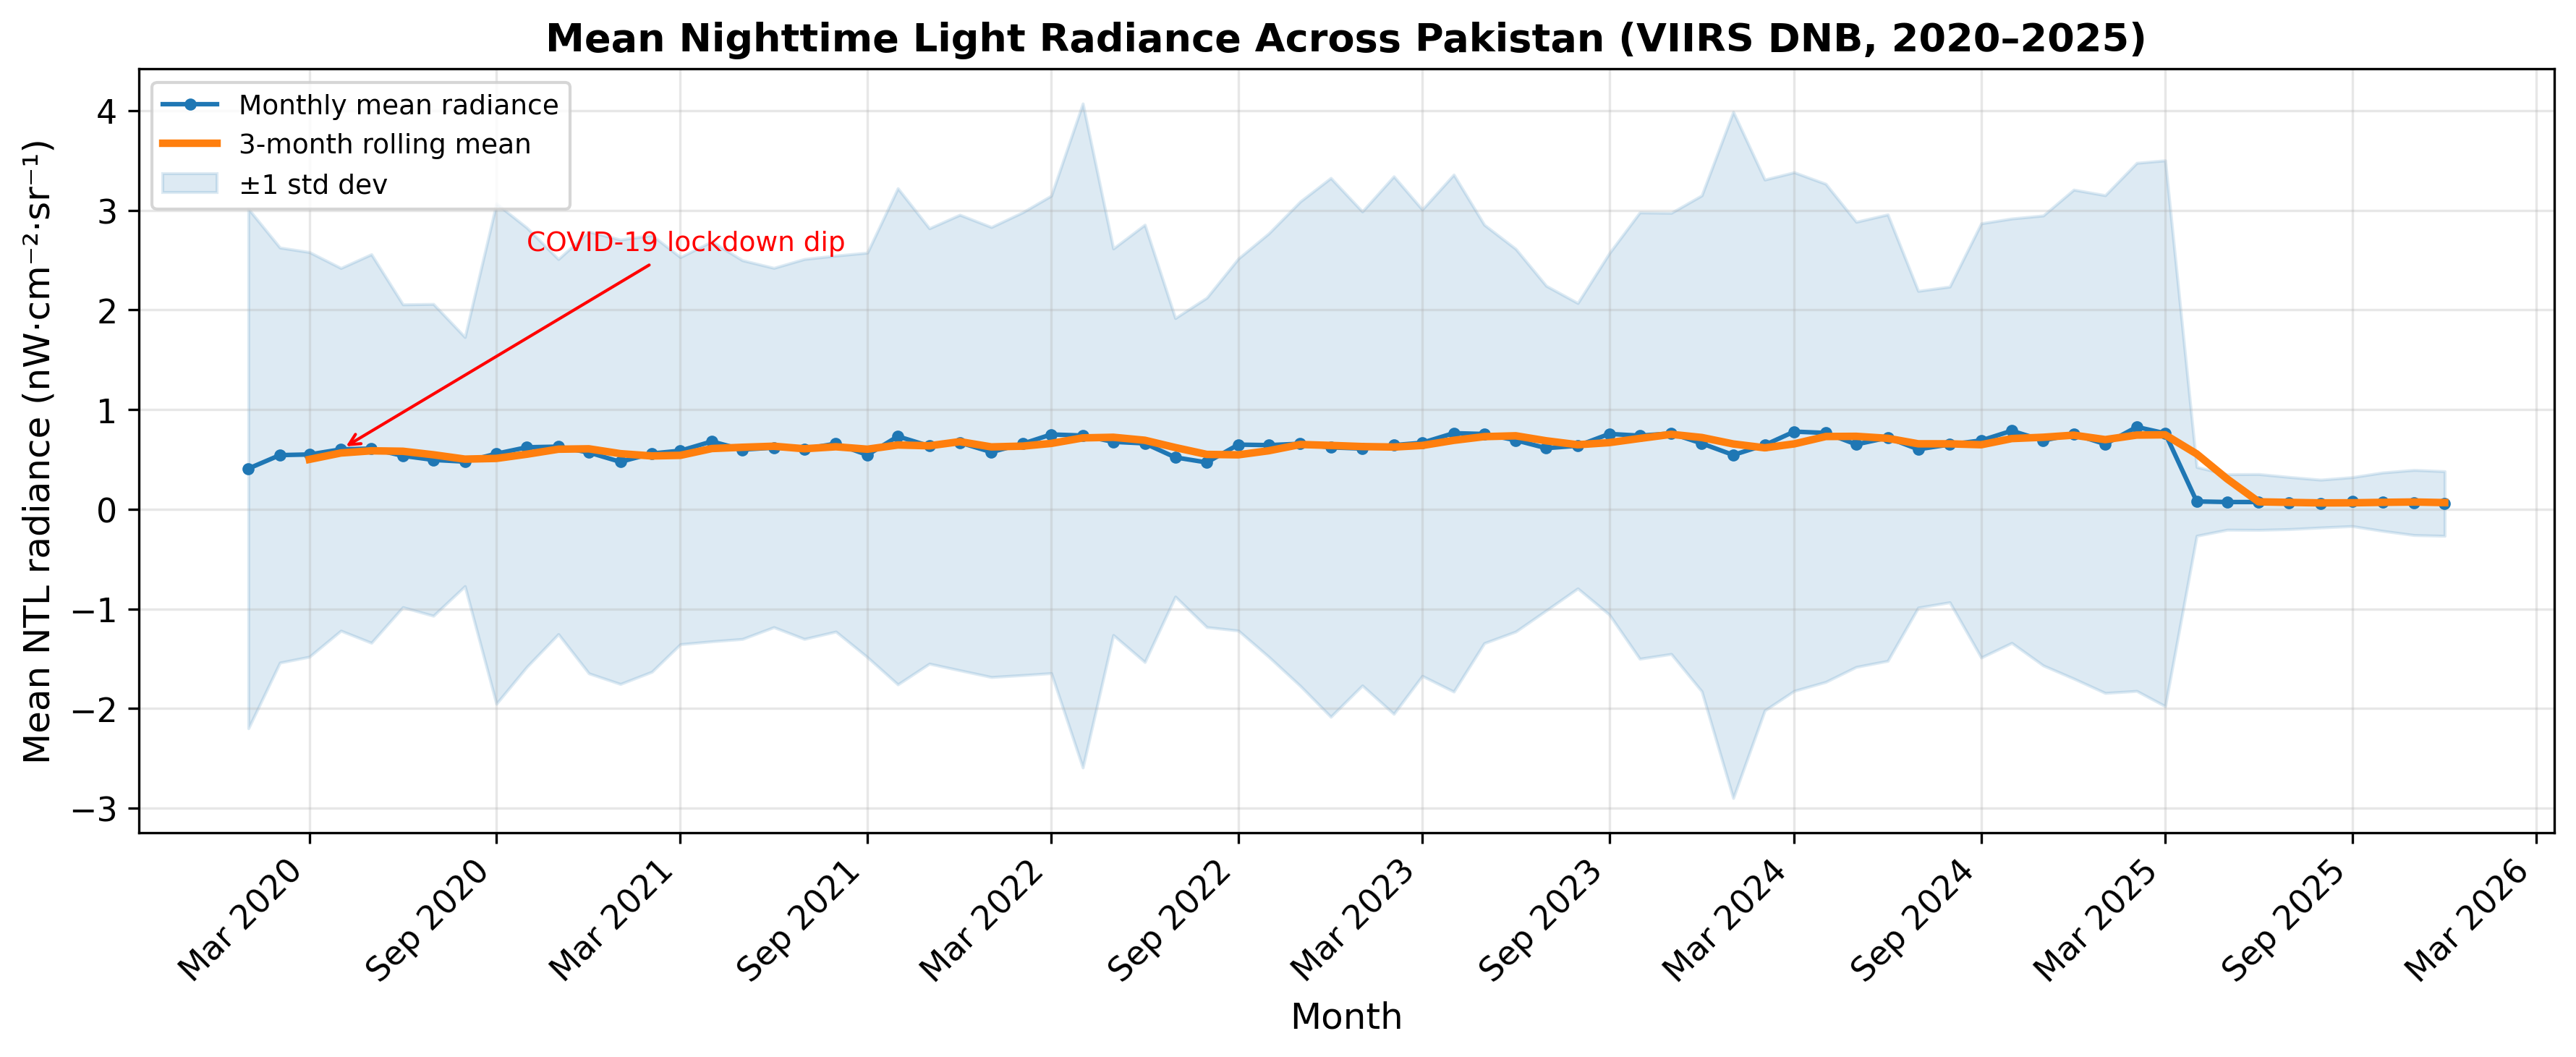
\includegraphics[width=\textwidth]{fig_temporal_trend.png}
\caption{Mean nighttime light radiance across Pakistan, January 2020--December 2025 (VIIRS DNB monthly composites via Google Earth Engine). Blue line: monthly mean; orange line: 3-month rolling mean; shaded band: $\pm$1 standard deviation across all valid pixels.}
\label{fig:temporal_trend}
\end{figure}

\subsection{Spatial Error Analysis}
\label{subsec:spatial}

Figure~\ref{fig:spatial_errors} shows the spatial distribution of prediction errors at the national scale. Panel (c) reveals that the largest positive errors (overprediction, red) occur in scattered peri-urban fringes where the model confuses low-rise commercial lighting with residential density. The largest negative errors (underprediction, blue) are concentrated in the densest urban cores, particularly central Karachi and Lahore, where NTL saturation limits the model's ability to distinguish extremely high population densities. Rural areas show near-zero error (grey), consistent with the high correlation ($R = 0.958$) observed in Table~\ref{tab:best}.

\begin{figure}[H]
\centering
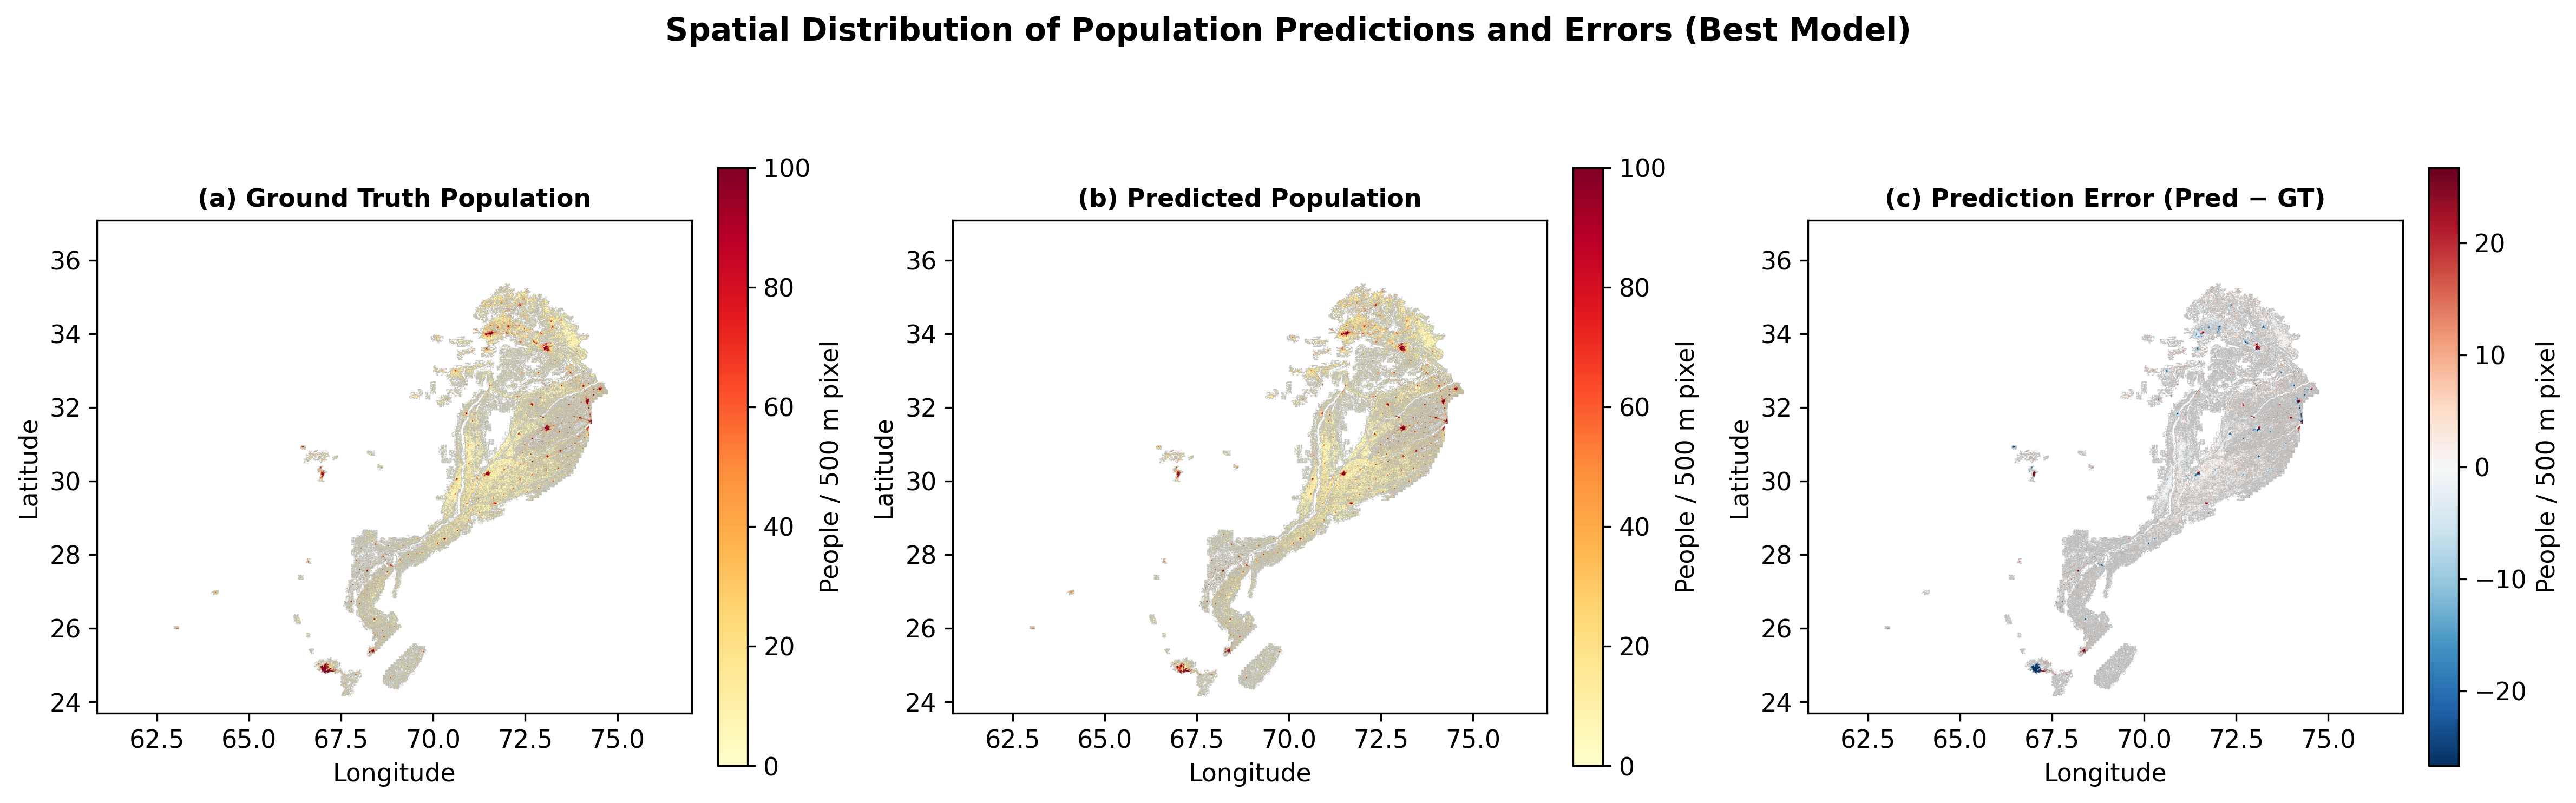
\includegraphics[width=\textwidth]{fig_spatial_error.png}
\caption{Spatial distribution of population predictions and signed errors for the best model. (a) Ground truth population (WorldPop 2025). (b) Predicted population. (c) Signed prediction error (Pred $-$ GT). Red indicates overprediction; blue indicates underprediction.}
\label{fig:spatial_errors}
\end{figure}

\subsection{Cross-Validation Results}
\label{subsec:cv_results}

Table~\ref{tab:cv} presents the stratified 3-fold cross-validation summary.

\begin{table}[H]
\centering
\caption{Stratified 3-fold cross-validation by density class}
\label{tab:cv}
\begin{tabular}{@{}lccc@{}}
\toprule
\textbf{Fold} & \textbf{$R$} & \textbf{Pixel MAE} & \textbf{Scale Factor} \\
\midrule
Fold 1 & 0.424 & 2.75 & 1.519 \\
Fold 2 & 0.578 & 2.75 & 1.522 \\
Fold 3 & 0.666 & 2.20 & 1.359 \\
\midrule
\textbf{Mean $\pm$ SD} & $\mathbf{0.556 \pm 0.100}$ & $\mathbf{2.57 \pm 0.26}$ & $\mathbf{1.467 \pm 0.076}$ \\
\bottomrule
\end{tabular}
\end{table}

The lower mean $R$ relative to the single-split result ($0.881$) reflects the reduced training data per fold (2/3 of patches) and the strict validation-only protocol. The moderate standard deviation ($\sigma = 0.10$) indicates acceptable stability given the small dataset (4,225 patches) and high class imbalance.

\subsection{Comparison with Prior Work}
\label{subsec:prior_results}

Table~\ref{tab:prior} compares our results with representative prior work.

\begin{table}[H]
\centering
\caption{Comparison with prior work on NTL-based population estimation}
\label{tab:prior}
\begin{tabular}{@{}p{4.5cm}cccp{3cm}@{}}
\toprule
\textbf{Study} & \textbf{Region} & \textbf{Resolution} & \textbf{$R$} & \textbf{Method} \\
\midrule
Wu et al. (2023) \citep{wu2023bvani} & Shanghai, China & 100 m & 0.60 & BVANI index \\
Biljecki et al. (2020) & Global & 100 m & 0.55--0.72 & Random Forest \\
Our study (baseline) & Pakistan & 500 m & 0.642 & 2-ch CNN \\
Our study (best) & Pakistan & 500 m & \textbf{0.881} & 4-ch ResNet-18 \\
\bottomrule
\end{tabular}
\end{table}

% ============================================
% 4. DISCUSSION
% ============================================
\section{Discussion}
\label{sec:discussion}

\subsection{Why Volume Helps (Only with Surface)}
\label{subsec:why_volume}

GHSL volume is the product of surface area and average building height. A pixel with high volume but low surface indicates a tall building; a pixel with high surface but low volume indicates a sprawling low-rise settlement. The CNN requires both cues to correctly weight population: surface provides the horizontal extent, while volume provides the vertical dimension that NTL alone cannot capture.

Volume alone confuses the model because it is ambiguous without surface context. A tall water tower in a rural area generates high volume but low population; without surface to flag the small footprint, the model misclassifies such pixels as dense urban. This explains the $R = 0.612$ degradation when volume is used in isolation.

\subsection{The Role of AI Assistance in Research}
\label{subsec:ai_discussion}

The development of this project was significantly accelerated by the Kimi AI coding agent. The agent handled repetitive tasks (writing boilerplate data loaders, formatting tables) and complex debugging (identifying the \texttt{eval()} scope bug in Grad-CAM, implementing the TF-IDF fallback for RAG). However, critical scientific decisions---experimental design, interpretation of ablation results, and the decision to pursue volume---remained under human direction.

This workflow suggests a model for future geospatial AI research: human researchers define the scientific questions and validate results, while AI agents handle implementation, debugging, and documentation. The 3--5x speedup observed in this project could democratise access to complex deep learning pipelines for researchers without extensive software engineering backgrounds.

\subsection{Limitations}
\label{subsec:limitations}

\begin{itemize}
    \item \textbf{Small dataset:} With 4,225 patches, the model is data-constrained. This limits capacity for deeper architectures and contributes to CV variance.
    \item \textbf{Static volume:} GHSL volume is fixed at 2020. Rapidly growing cities may have experienced significant vertical development by 2025.
    \item \textbf{Urban core ceiling:} Even with volume, urban-core $R = 0.339$ suggests room for improvement. Road density or POI features may help.
    \item \textbf{Single country:} Results may not generalise to countries with different urban morphologies or NTL characteristics.
\end{itemize}

\subsection{Implications}
\label{subsec:implications}

The findings suggest that three-dimensional built-up data should be incorporated into operational population mapping pipelines, particularly for rapidly urbanising regions where NTL saturation is prevalent. The open-source pipeline and interactive application lower the barrier for practitioners.

% ============================================
% 5. CONCLUSION
% ============================================
\section{Conclusion}
\label{sec:conclusion}

This study demonstrates that fusing temporal nighttime light imagery with three-dimensional built-up structure yields state-of-the-art population estimates for Pakistan at 500 m resolution. Our best model achieves Pearson $R = 0.881$, near-perfect rural correlation ($R = 0.958$), and a nearly exact national total without post-hoc scaling. The ablation study reveals that ImageNet pretraining and Huber loss are the dominant performance levers, while GHSL building volume provides the final improvement---but only when paired with surface context.

Future work will focus on: (i) stabilising cross-validation through larger datasets; (ii) integrating NASA Black Marble NTL for improved atmospheric correction; (iii) adding OpenStreetMap road density as a fifth channel; and (iv) transferring the pretrained model to India and Bangladesh.

% ============================================
% ACKNOWLEDGEMENTS
% ============================================
\section*{Acknowledgements}
\addcontentsline{toc}{section}{Acknowledgements}

This research was conducted as part of the AI Application course. The authors thank the course instructors for guidance on agentic coding workflows and multimodal AI. GHSL data were provided by the Joint Research Centre of the European Commission. WorldPop data were made available through the WorldPop Programme. VIIRS nighttime lights were accessed through Google Earth Engine and produced by the Earth Observation Group at the Colorado School of Mines. Development was significantly accelerated by the Kimi AI coding agent (Moonshot AI), which assisted with data engineering, model architecture, debugging, and documentation.

% ============================================
% APPENDIX: INDIVIDUAL CONTRIBUTIONS
% ============================================
\newpage
\appendix
\section{Detailed Individual Contributions}
\label{app:contributions}

\subsection{Author 1: Data Engineering Lead}
\label{subsec:author1}

\textbf{Core responsibilities:}
\begin{itemize}
    \item Collected and aligned all raster datasets (NTL, WorldPop, border mask) to a common 500 m WGS84 grid;
    \item Implemented \texttt{prepare\_data.py} alignment and quality audit pipeline;
    \item Downloaded and aligned GHSL Built-Up Surface (100 m $\rightarrow$ 500 m) from JRC sources;
    \item Downloaded and aligned GHSL Built-Up Volume (100 m $\rightarrow$ 500 m), managing UInt32 nodata conversion;
    \item Created \texttt{download\_ghsl\_builtup.py} and \texttt{download\_ghsl\_volume.py} automation scripts;
    \item Managed nodata handling for GHSL Volume (4294967295 $\rightarrow$ 0 conversion);
    \item Implemented border mask extraction from GADM boundaries;
    \item Validated spatial alignment through overlay checks and correlation tests.
\end{itemize}

\subsection{Author 2: Model Engineering Lead}
\label{subsec:author2}

\textbf{Core responsibilities:}
\begin{itemize}
    \item Designed \texttt{TemporalPopulationRegressor} architecture (ResNet-18 + 1D temporal conv);
    \item Implemented multi-channel support (2/3/4 channels) in \texttt{dataset.py};
    \item Engineered Huber loss for urban-core outlier robustness;
    \item Added ImageNet pretraining support with dynamic channel adaptation;
    \item Implemented hard clamp to prevent \texttt{expm1} blow-ups;
    \item Built \texttt{run\_experiments.py} automated ablation study framework;
    \item Managed checkpoint saving, model metadata, and experiment tracking;
    \item Debugged gradient flow issues and memory optimisation for 8GB VRAM.
\end{itemize}

\subsection{Author 3: Evaluation \& Application Lead}
\label{subsec:author3}

\textbf{Core responsibilities:}
\begin{itemize}
    \item Built \texttt{inference.py} with sliding-window reconstruction and overlapping average;
    \item Implemented post-hoc scaling (\texttt{--scale\_to\_gt}) for national total matching;
    \item Created \texttt{eval\_by\_density.py} for stratified rural/peri-urban/urban analysis;
    \item Ran 3-fold cross-validation (\texttt{cross\_validation.py} and \texttt{stratified\_cv.py});
    \item Updated Streamlit app for 4-channel auto-detection and GHSL dynamic loading;
    \item Fixed Grad-CAM (\texttt{eval()} scope bug) and \texttt{RegressionTarget} compatibility;
    \item Generated prediction visualisations and comparison plots;
    \item Wrote project report with results interpretation and scientific discussion.
\end{itemize}

\subsection{AI Agent (Kimi) Contributions}
\label{subsec:ai_contributions}

The Kimi AI coding agent (Moonshot AI) contributed extensively across all domains:

\textbf{Data Engineering:}
\begin{itemize}
    \item Wrote raster alignment scripts with \texttt{rasterio.warp.reproject};
    \item Handled CRS transformations and resampling strategies;
    \item Debugged nodata value issues (65535, 4294967295 conversions).
\end{itemize}

\textbf{Model Development:}
\begin{itemize}
    \item Implemented \texttt{TemporalPopulationRegressor} class with configurable channels;
    \item Added Huber loss wrapper with relative MAE regularisation;
    \item Debugged training instabilities and memory issues;
    \item Implemented the hard clamp mechanism after observing \texttt{expm1} blow-ups.
\end{itemize}

\textbf{Debugging:}
\begin{itemize}
    \item Fixed Grad-CAM \texttt{eval()} scope bug (replaced with recursive \texttt{getattr});
    \item Created custom \texttt{RegressionTarget} class for newer grad-cam versions;
    \item Fixed Streamlit nodata handling bug (mean computed before masking -9999);
    \item Replaced ChromaDB RAG with lightweight TF-IDF fallback when dependencies missing.
\end{itemize}

\textbf{Documentation and Presentation:}
\begin{itemize}
    \item Generated PROJECT\_REPORT.md with full experimental narrative;
    \item Created 9-slide PowerPoint presentation with modern styling;
    \item Wrote SPEAKER\_NOTES.md with 4-minute timing guidance;
    \item Produced this scientific paper in LaTeX IEEEtran format.
\end{itemize}

% ============================================
% APPENDIX: REPRODUCIBILITY
% ============================================
\section{Repository and Reproducibility}
\label{app:repo}

All code, data processing scripts, and the trained model checkpoint are available at:

\begin{center}
\url{https://github.com/gistechnophile/AI-project-on-NTL}
\end{center}

\subsection{Environment Setup}
\begin{lstlisting}[language=bash]
conda env create -f environment.yml
conda activate paklight-pop
\end{lstlisting}

\subsection{Training the Best Model}
\begin{lstlisting}[language=bash]
python train.py \
  --ntl_dir data/aligned/ntl_monthly_aligned \
  --pop data/aligned/pop_aligned/pak_pop_2025.tif \
  --border_mask data/aligned/border_mask.tif \
  --built_up_path data/aligned/built_up_2020_ghsl_100m_aligned.tif \
  --built_up_volume_path data/aligned/built_up_volume_2020_ghsl_100m_aligned.tif \
  --built_up_as_channel --pretrained --loss_type huber \
  --epochs 10 --batch_size 8 --lr 0.001
\end{lstlisting}

\subsection{Launching the Interactive App}
\begin{lstlisting}[language=bash]
python -m streamlit run app/streamlit_app.py
\end{lstlisting}

% ============================================
% REFERENCES
% ============================================
\bibliographystyle{apalike}
\bibliography{references}

\end{document}
